\section{Porta Design and Implementation}

The goal of Porta is to give tutorial creators an efficient way to see
how learners actually progress through their instructional materials and
where they might have struggled. It is meant to be activated during a
user testing session where the participant's task is to follow the steps
in a given tutorial.

Porta automatically records relevant actions with no user intervention.
At the end of the session, Porta produces a visualization summarizing
the participant's actions during each part of the tutorial.
%
In this way, \emph{Porta facilitates user testing of tutorials and other
technical documentation} rather than traditional user testing of
software artifacts.
%
It consists of three components: 1)~an operating-system-wide application
usage profiler, 2)~a web browsing tracker, and 3)~a profiling
visualization that augments the original tutorial webpage.


\subsection{OS-Wide Application Usage Profiler}

Porta's OS-wide usage profiler allows it to transparently monitor user
activity across multiple applications. Our prototype is implemented for
macOS using AppleScript, Python, Bash, and DTrace~\cite{Cantrill2004} scripts; but
the concept is OS-independent.

%It should be straightforward to port this OS-wide tracing approach to
%other operating systems.

When user-testing a tutorial, the participant first launches this
profiler in the background before starting to work through the steps on
the tutorial webpage. It continually monitors the following data and
records it to a JSON-formatted log. All monitored events are
timestamped, so in aggregate they form a unified cross-application usage
profile.

%which can later be visualized alongside the original tutorial webpage's
%contents.

\begin{itemize}

    \item \textbf{Screencast video}: Apple's built-in Quicktime app is
    used to record a video of the participant's entire screen, system
    audio, and spoken audio via the built-in microphone. This is
    important for showing the participant's actions within GUI-based
    applications as they follow a tutorial.

    \item \textbf{Clipboard}: When the participant copies text to the
    clipboard, its contents are logged. This can show what they
    copied-pasted from tutorials into other apps such as IDEs.

    \item \textbf{Shell command invocations}: Porta installs a wrapper
    script that logs the timestamps and arguments of all shell commands
    invoked within terminals. It also logs the current directory and
    environment variables used for running each command. This logger
    works for Bash (default on macOS) and zsh, but can easily be
    extended to other shells.

    \item \textbf{Compiler/interpreter toolchain invocations}: In
    addition to logging all shell commands, Porta performs deeper tracking
    when the participant invokes compilers, interpreters, and other
    build tools (e.g., \texttt{make}, \texttt{webpack}) as they are
    following a tutorial. This is important for pinpointing which
    parts of a tutorial caused the participant to make code errors and
    tracking certain actions within IDEs.

    Specifically, Porta records the command-line arguments of each tool
    invocation. It also tracks all the files read by the processes and
    its forked subprocesses, which are usually the relevant source code
    files that are compiled or executed. Finally, it records the
    invocation's textual output (on both stdout and stderr), as well as
    the error return code, which indicates either a successful or
    erroneous execution.

    To accomplish this tracking in an application-agnostic way, when
    Porta is first activated it automatically generates wrapper scripts for toolchain
    executables such as \texttt{gcc}, \texttt{make}, \texttt{node},
    \texttt{javac}, and \texttt{python} (in a user-customizable list).
    It adds the directory of those wrappers to the start of the
    \texttt{\$PATH} environment variable so that they can be invoked
    in an identical manner as the original apps.

    When a wrapper script is invoked, it forks a child process to run
    the original executable with identical command-line arguments. It connects
    stdin, stdout, stderr streams so that it behaves identically to the original,
    and also logs the child's stdout/stderr outputs to a file.
    %
    It then launches DTrace~\cite{Cantrill2004} to record \texttt{fopen}
    system calls issued by that child and any of its children. These
    system calls indicate which files the toolchain invocation is taking
    as inputs (e.g., Makefiles, source code files). Porta saves a copy
    of those files in its log directory on each invocation. It ignores
    binary files (e.g., system libraries) by filtering using MIME types~\cite{mime}.

    DTrace is necessary here since it is impossible to tell what files
    are accessed by a command solely by inspecting its command-line
    arguments. For instance, running the command \texttt{python
    foo.py} reads in not only \texttt{foo.py} but also all files that
    are dynamically imported by its code.

    Another major benefit of this wrapper- and DTrace-based
    approach is that it works regardless of whether these
    tools are invoked from the terminal or within an IDE. For instance,
    when the user presses the ``Compile" or ``Run" button in an IDE, that will invoke the operating
    system's compiler/interpreter executables, which will call the
    wrapper versions since those appear first in the user's
    \texttt{\$PATH}.

    \item \textbf{Remote activity tracing via \texttt{ssh} invocations}:
    Many kinds of technical tutorials involving system administration,
    web development, and cloud-based execution will require users to run
    commands on remote servers. To support remote tracking, Porta
    replaces the built-in \texttt{ssh} executable with a wrapper that
    injects a shell script into the remote machine when the participant
    first logs into that machine.

    This injected script lets Porta monitor command invocations on the
    remote machine in an identical manner as on the participant's local
    machine. It supports logging into both macOS and Linux servers.
    Porta uses a Linux port of
    DTrace to achieve the same kind of toolchain invocation
    tracing as it does for macOS~\cite{dtrace4linux}. In the future, we can also port the
    tracer to Windows using its Process Monitor~\cite{procmon}.

    The ssh script also injects a unique session ID into each login
    session. This allows Porta to properly group remote toolchain
    invocations into sessions in cases when the participant either logs
    into multiple servers or to the same server using different terminal
    shells. When the user logs out at the end of each session, the ssh
    script copies the log file from the server back to the participant's
    local machine.

\end{itemize}

Note that the related Torta system~\cite{MysoreUIST2017} contains
similar screencast video and shell command recorders, but all other
components described in this paper are not in Torta. Also, the goal of
our Porta system differs from those of prior application profilers:
Porta's novelty lies in combining this data with web browser tracking
(next section) to create \emph{tutorial profiles}.


\subsection{Web Browsing Activity Tracker}

\begin{figure}
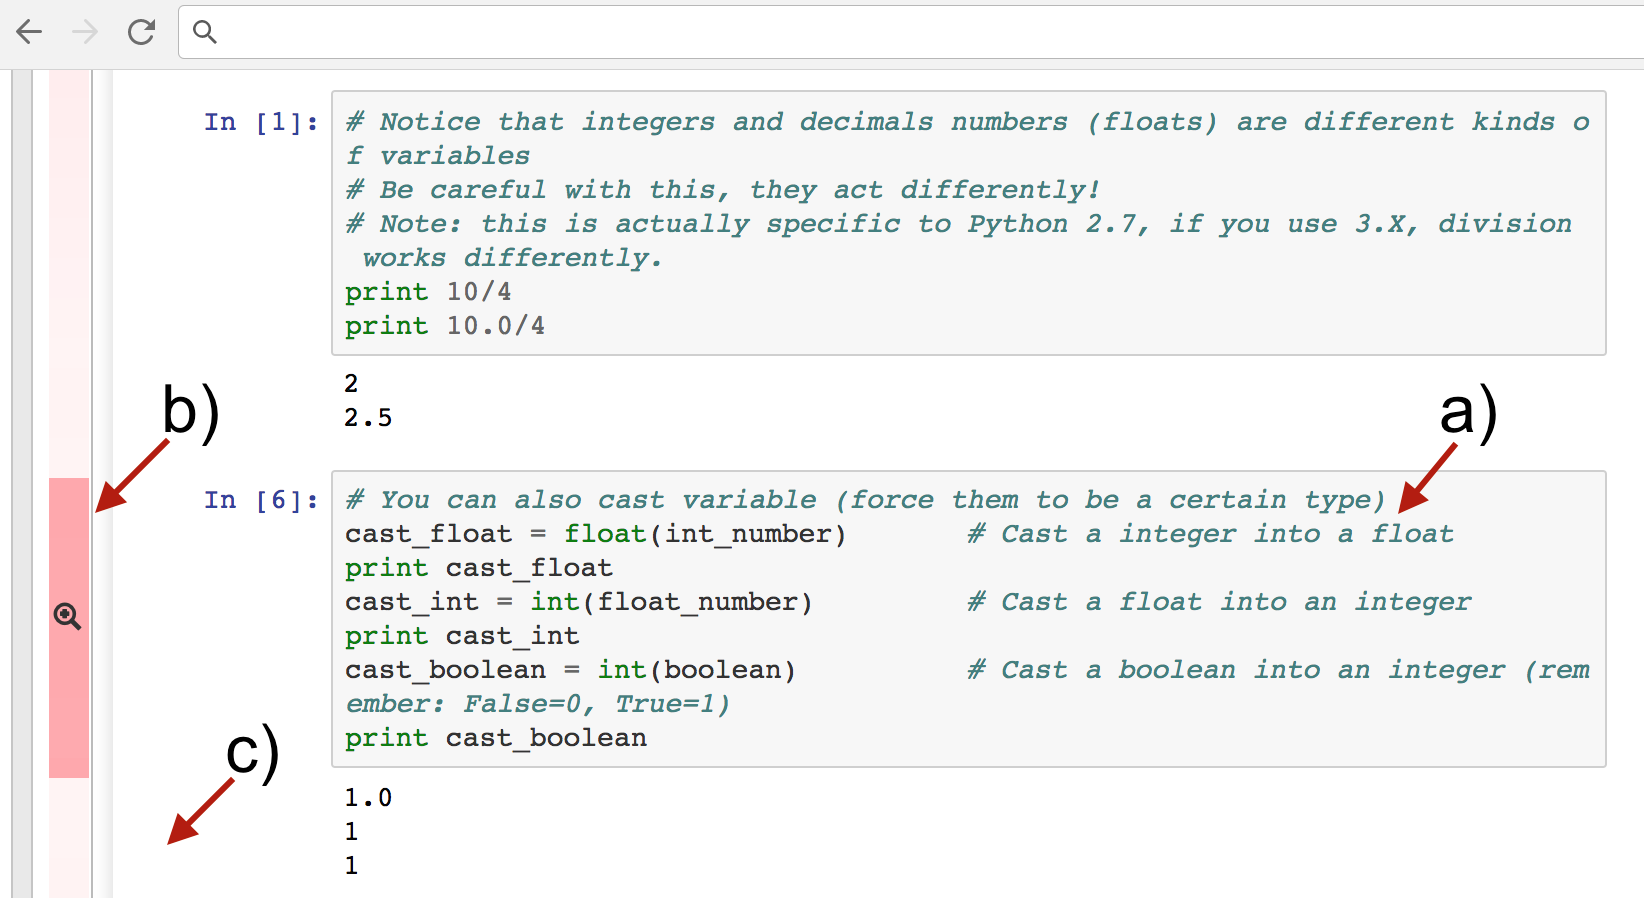
\includegraphics[width=\columnwidth]{figures/porta/mouse-hover.png}
\vspace{-0.5em} % stent
\caption{Porta uses mouse location as a proxy for where the user's
attention is focused. a) If the user hovers over anywhere in this code
block element, Porta will record it as being in focus and b) render it
as a red hotspot in the sidebar heatmap. c) If the user hovers over an
element (e.g., background) that is larger than the viewport, that event
is ignored.}
\label{fig:browser-tracking}
\vspace{-0.25em} % stent

\end{figure}

Porta also tracks detailed user activity within web browsers using a
Google Chrome extension.

The participant activates this extension when they are about to start
following a tutorial presented on a given webpage. It tracks a
timestamped log of the following browser-related activities:

    \begin{itemize}

        \item \textbf{Hover-focused webpage element}: The web tracker
        continually records the mouse position in terms of the most
        precise CSS path of the DOM element that the participant's mouse is
        currently hovering over (\fig{fig:browser-tracking}). This provides a rough indicator of what
        their attention is focused on at each moment. Ideally we
        would gather data from an eyetracker to determine the
        participant's true visual focus, but mouse hover is an
        approximation that is commonly used in commercial web
        analytics tools such as FullStory~\cite{fullstory}, Hotjar~\cite{hotjar},
        and Mouseflow~\cite{mouseflow}.

        (Our profile visualizations are designed to account for this
        level of imprecision.)

        This tracker ignores mouse events over elements that are larger
        than the browser's viewport (\fig{fig:browser-tracking}c). These positions likely
        indicate that the mouse is hovering over a webpage
        background element, which is a weaker indicator of focus,
        so the tracker conservatively ignores them. It also does not log
        mouse locations over non-browser windows.

        On the other extreme, when the mouse is hovering over an element
        that is too small (smaller than $10\times10$ pixels), the
        tracker traverses upward in the DOM to the first parent element
        larger than this minimum size threshold. This heuristic helps
        ensure it logs that the mouse is hovering over a non-trivial
        element such as a block of text or an embedded video rather
        than, say, a tiny stylistic component in the foreground that is
        occluding more meaningful content.

        Finally, to ignore noisy log entries due to mouse jitter, the
        tracker does not log an event until the mouse has hovered over a
        particular element for at least 0.5 seconds.

        Why not simply record raw x-y mouse positions? Because the goal
        of this tracker is to determine what meaningful page component
        the user is focusing on at each moment. For example, in
        \fig{fig:browser-tracking}a, it does not matter whether the user's mouse
        is over the left or right half of the code block element;
        we want to record that they are likely focused on that element
        at the moment. Another benefit of recording DOM elements
        rather than raw x-y positions is that the former is robust to
        browser window resizing, which can cause elements to shift to
        different x-y positions.

        In the end, short of directly asking the user what they are
        focusing on at each moment in the tutorial, all approximations
        are imperfect. Even eyetrackers produce noisy data as eye gazes
        wander and jitter~\cite{tobii2011}. We wanted to design a simple tracker that
        works in regular browsers without special equipment, so we
        adopted this mouse-based approach.

        \item \textbf{Scroll position and viewport size}: The tracker
        records the current scroll position of the participant in each
        tab, along with the browser's viewport size. This provides a
        coarser indicator of where the participant may be currently
        reading. We assume that if they are reading a webpage, they
        must be looking at content that is within view of the range
        defined by the current scroll position and viewport size.
        (However, we can never know for sure whether the participant is
        actually reading the tutorial at any given moment.)

        \item \textbf{State of embedded video players}: Technical
        tutorials sometimes embed short videos alongside their textual
        content, perhaps to play a mini-lecture, to demonstrate GUI
        operations, or to show a screencast of code being written and
        executed. Porta
        records all events on video player components embedded within
        webpages, such as play, pause, stop, and seek events, along with
        their seek positions. This tracer uses the browser's built-in
        HTML5/JavaScript video API, which works with all modern
        non-Flash videos including, most commonly, embedded YouTube videos.
       
        \item \textbf{Opening webpages}: The tracker records
        the timestamp and URL of every tab and browser window opened by
        the participant. This is important because they might open new
        tabs to search for topics in the tutorial that are hard for them
        to understand, so Porta should track when they do so.

        \item \textbf{Opening Chrome developer tools}: It also records
        the tabs in which the participant has opened the browser's
        developer tools pane, which contains a JavaScript console,
        HTML/CSS inspector, network inspector, and JavaScript debugger.
        This action signals that they may be trying to follow some kind
        of web development tutorial and are currently debugging their
        web-related code in that tab.

        \item \textbf{JavaScript errors}: Finally, the tracker logs all
        JavaScript errors on webpages where the participant has opened
        the developer tools to presumably debug their web-related code
        while following a tutorial. In addition, errors are always
        logged for pages on the localhost domain, even without opening
        developer tools, since those are likely pages that the
        participant is editing and debugging locally while following a
        web development tutorial. This within-browser logging is similar
        to Porta logging the error messages produced by
        compiler/interpreter toolchain invocations.

\end{itemize}

Although profiling user activity within webpages is not a new idea
(commercial analytics tools do some form of this~\cite{fullstory,hotjar,mouseflow}), the
main novelty of Porta lies in combining web tracking with the
application usage profiler from the prior section to create novel
\emph{tutorial profiling visualizations}.


\subsection{Tutorial Profiling Visualizations}

\begin{table}

\small
\begin{tabular}{l}
%\toprule

\\[-1em]
\underline{OS-Wide Application Usage Profiler} \\
%\hline

Screencast video (fullscreen audio/video recording of test session) \\

Clipboard text (for tracking copy-paste actions) \\

Shell commands (all commands run in Bash/zsh in any terminal) \\

Toolchain invocations (run from shell or within an IDE) \\

Remote ssh invocations (shell/toolchain commands on remote servers) \\

\\[-0.4em]
\underline{Web Browsing Activity Tracker} \\
%\hline

Hover-focused webpage element (use mouse as proxy for user focus) \\

Scroll position and viewport size \\

Embedded video player state (all HTML5 players including YouTube) \\

Opening webpages \\

Opening Chrome developer tools \\

JavaScript errors \\

\end{tabular}

\caption{Summary of trace data that is automatically collected by Porta's OS-wide and within-browser trackers. All events are timestamped.}

\label{tbl:tracers}

\end{table}


\tab{tbl:tracers} summarizes the data that Porta automatically collects
on the participant's computer as they follow a tutorial during a testing
session. Porta combines all this data into a tutorial profiling
visualization, which can be used in two main ways:

\begin{itemize} \itemsep0pt

\item The test facilitator shows it to the participant in a post-study
debriefing so that the participant can see where they struggled and
better reflect on why they took those actions.

\item Porta can aggregate the trace data from a group of test users and
present it to the tutorial's creator so that they can see where people
collectively struggled.

\end{itemize}

In both use cases, the ultimate goal is to provide feedback to the
tutorial's creator so that they can improve its contents.


\textbf{Heatmap visualizations}:
%
\fig{fig:porta-components} shows that Porta displays tutorial profiles
as positional and temporal heatmaps alongside the left and bottom of the
tutorial webpage, respectively.
%
The right half of \fig{fig:porta-overview} shows this UI on a real webpage.

We implemented this visualization as a web application that embeds the
original tutorial webpage in an iframe. We took this iframe-based
approach so that we do not need to modify the tutorial webpages. In
earlier iterations of Porta, we injected DOM elements and JavaScript
events as an overlay atop webpages, but that was not robust; our
elements sometimes altered the layout of those pages or came into
conflict with frontend frameworks or libraries. Overlays also occluded
certain page elements. Using our iframe approach, the profiled webpages
appear exactly as how the test participant and tutorial creator
originally saw them.

The \emph{positional heatmap} shows where on the tutorial
webpage the participant was looking at the most, and what else they were
doing on their computer while looking at each part. Just like how a
source code profiler~\cite{Graham1982,Srivastava1994} shows \emph{hotspots} of lines of
code where the computer spent the most time executing, this heatmap
visualization shows hotspots of where participants spent the most time
while following a tutorial.


\begin{figure}
  \centering
  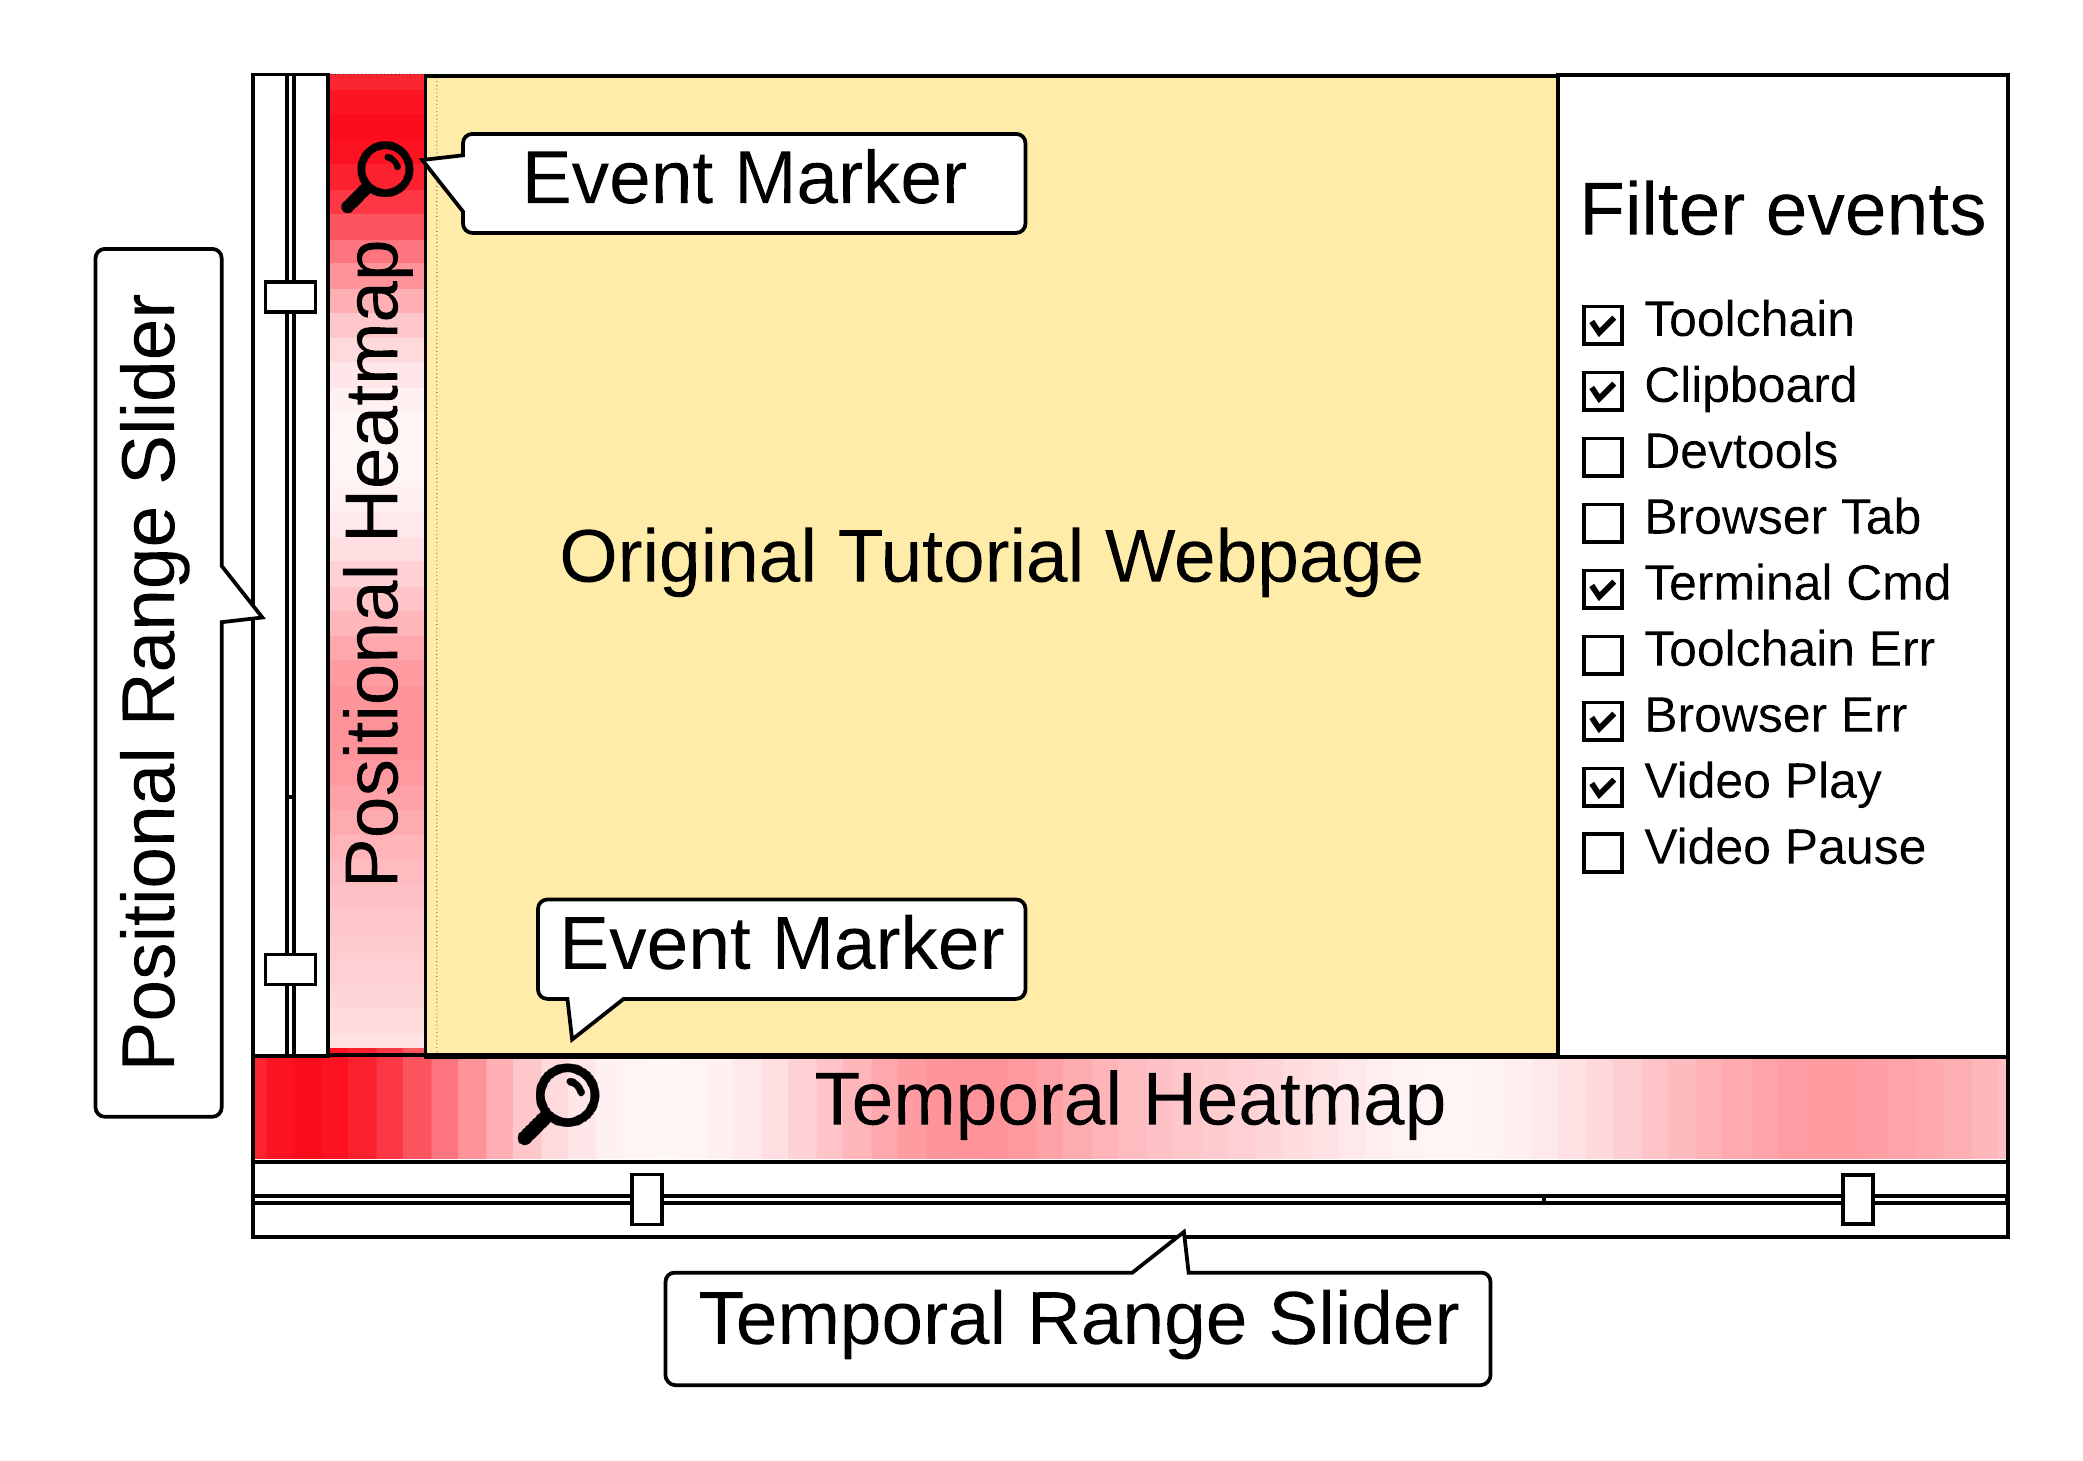
\includegraphics[width=0.9\columnwidth]{figures/porta/porta-viewer-sketch}

\vspace{-0.75em}

  \caption{Porta uses the trace data collected from test sessions to
  augment the original tutorial webpage with heatmap visualizations
  showing positional focus and temporal density of events. Specific
  occurrences of events show up as clickable markers on both heatmaps.}

\vspace{-0.75em}

  \label{fig:porta-components}
\end{figure}

\begin{figure}
  \centering
  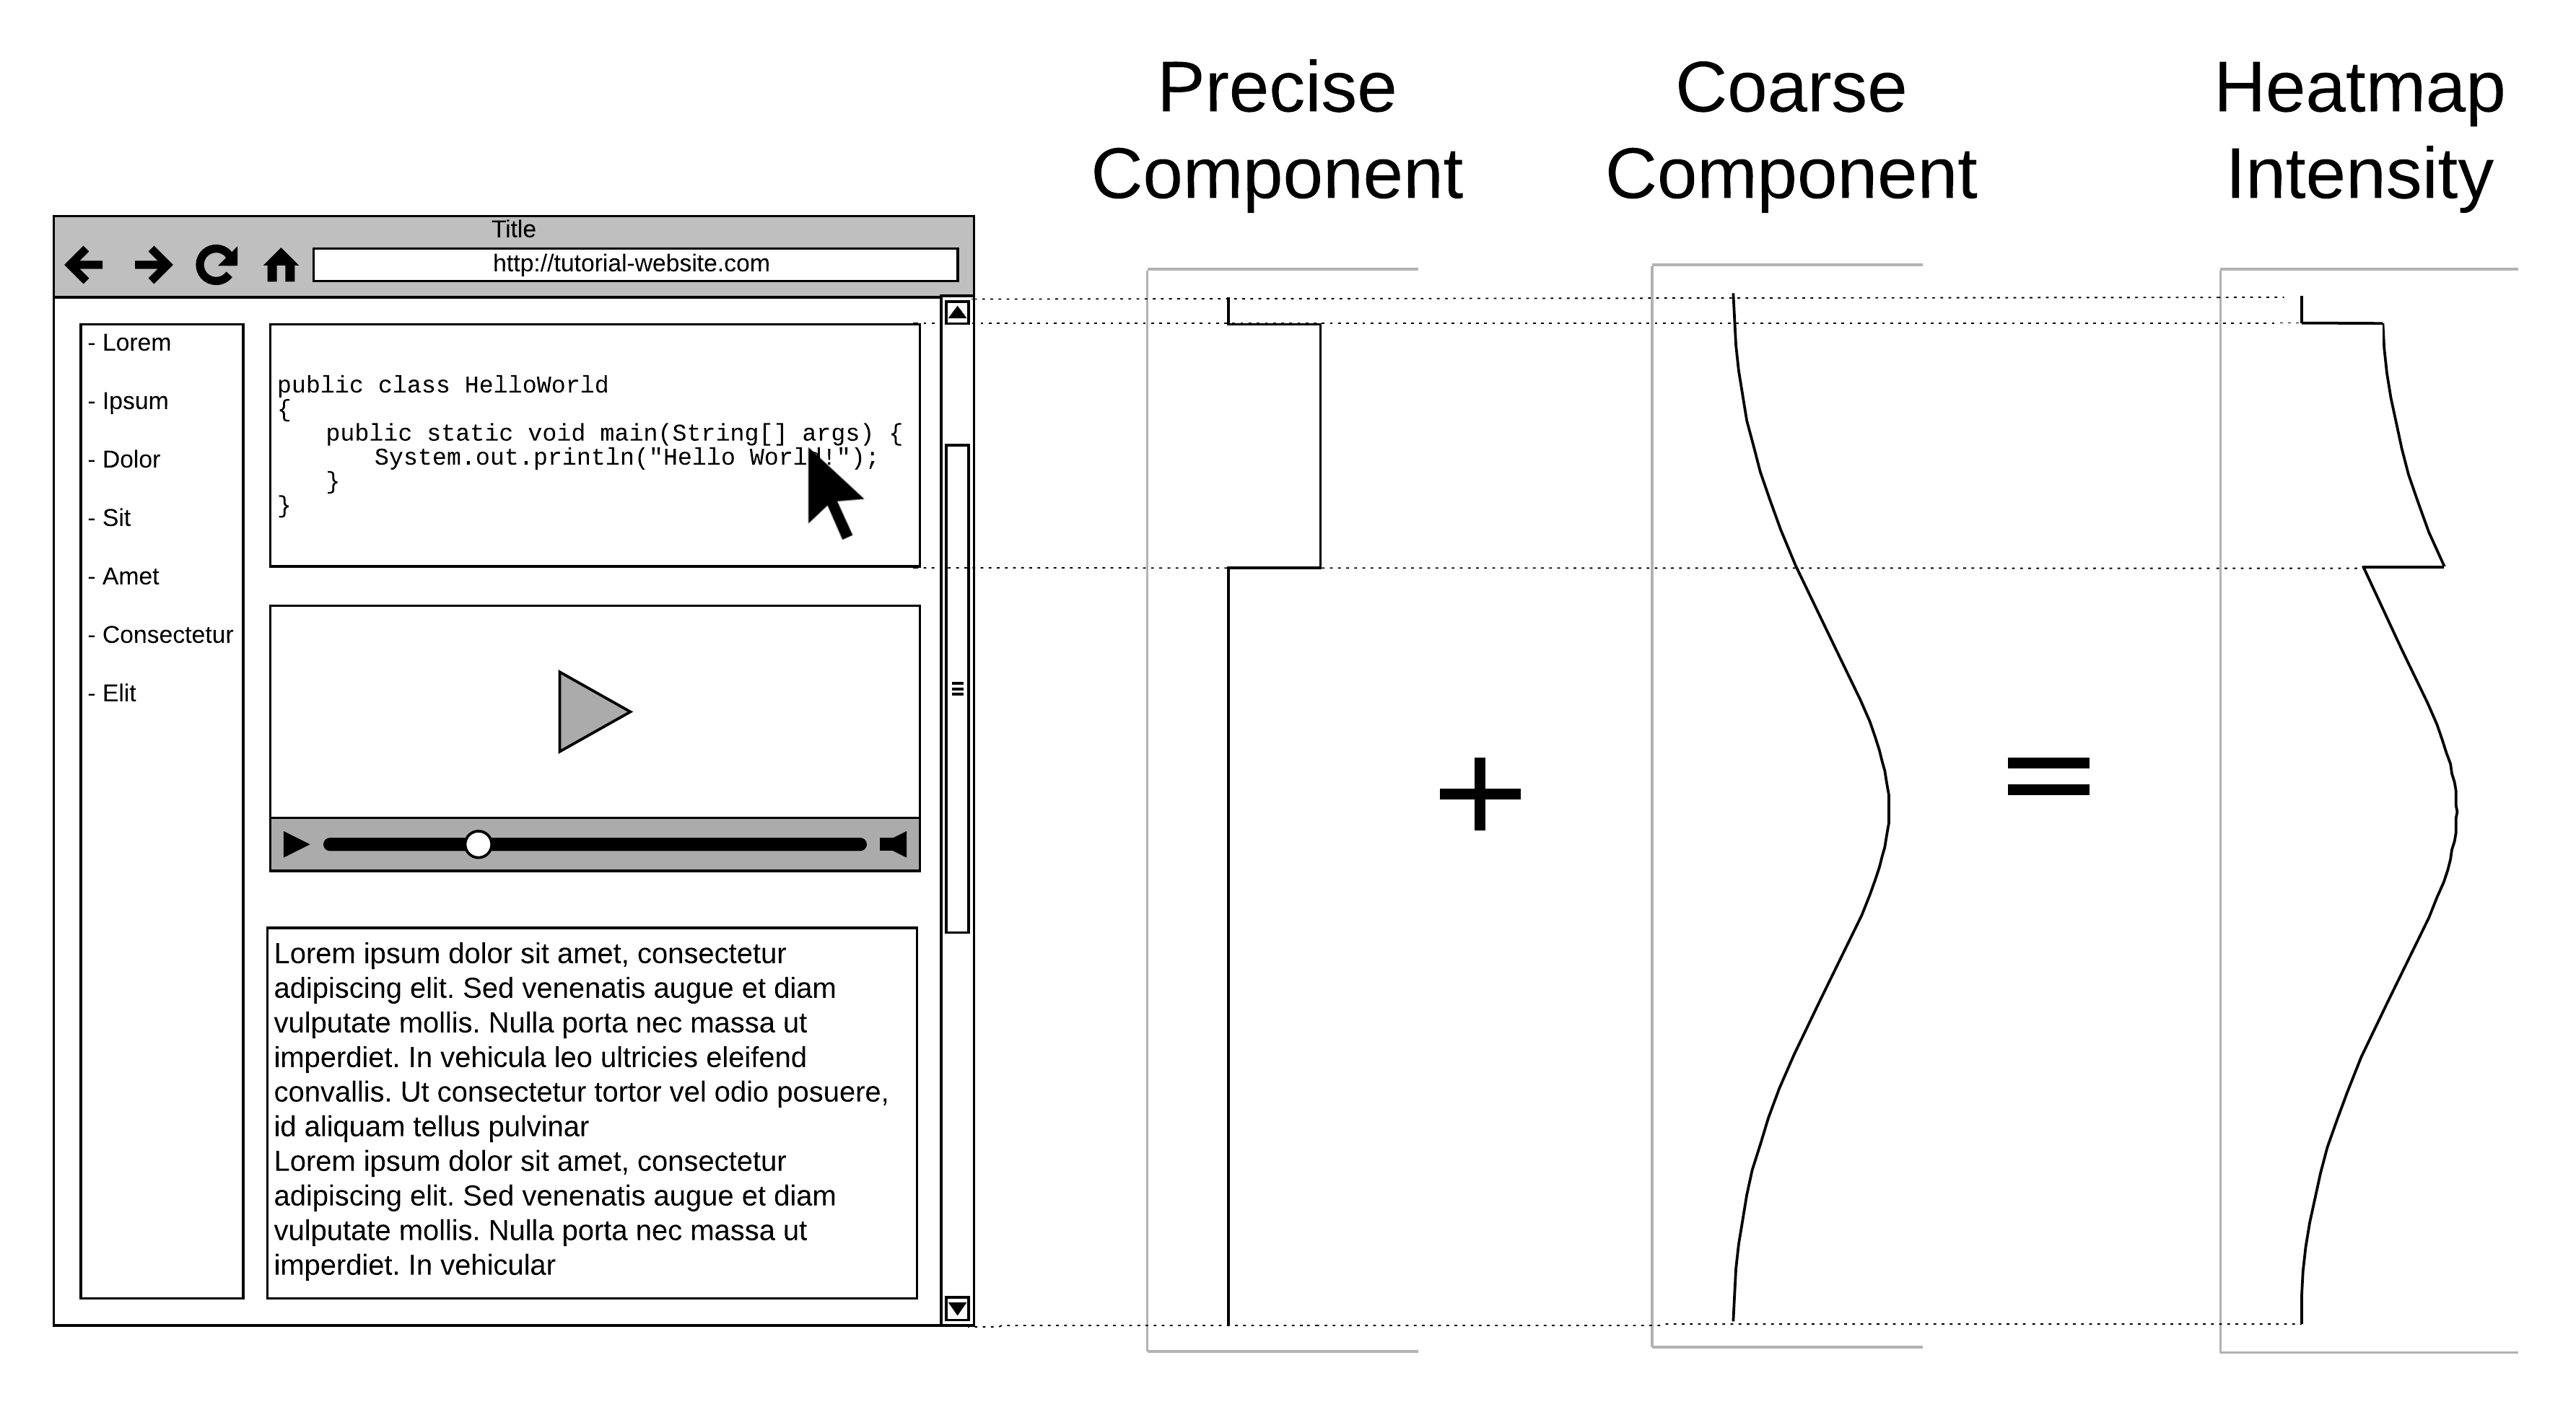
\includegraphics[width=0.9\columnwidth]{figures/porta/heatmap}

\vspace{-0.75em}

  \caption{The positional heatmap's intensity is a time-weighted sum of
  precise (mouse hovering over a specific DOM element) and coarse
  components (Gaussian centered at the middle of the viewport).}

  \label{fig:pos-heatmap}
  \vspace{-0.5em} % stent
\end{figure}


This heatmap shows the approximate amounts of time that the participant
spent on each vertical portion of the webpage throughout the session.
\fig{fig:pos-heatmap} shows how it is the time-weighted sum of two
components: 1)~a precise component based on mouse hover locations over
specific DOM elements, and 2)~a coarse component based on browser scroll
position and viewport size. For example, in \fig{fig:pos-heatmap}, the
mouse is hovering over an example code block, so the precise component
covers the entire height of that DOM element. However, we cannot be
certain that the participant is actually looking at that element; they
might have left the mouse there while reading other content on the page.
To account for this inherent uncertainty, we add a coarse component
consisting of a Gaussian distribution at the middle of the viewport. We
chose parameters to cover the viewport within 2 standard deviations
(95\% of the Gaussian's area). The assumption here is that the user is
more likely looking at the center rather than the edges.

%The heatmap intensity for that moment is a weighted sum of those
%components.

If the participant now moves their mouse away from the browser to
another application window such as their IDE, we can no longer use mouse
location as a proxy for their current focus. Thus, Porta instead relies
only on the coarse (Gaussian) component to approximate their focus
location.
%
If the browser window is occluded, that may decrease the chances that
they are looking at certain parts of the webpage, but we have not yet
accounted for this level of detail in our prototype.

To produce the positional heatmap for the entire session, Porta time-weighs the
computed values for each moment and maps them to a monochromatic
color scale to display a 1-D vertical heatmap along the
left side of the tutorial webpage. Since this is located in a separate
iframe, Porta synchronizes vertical scroll events and viewport size
changes between the tutorial webpage iframe and the heatmap's iframe so
both are always in sync regardless of page scrolling or resizing.
%
We chose a 1-D vertical heatmap since tutorials are usually formatted
vertically. This also matches the interface of code profilers, which
display vertically down an IDE's or text editor's gutter to show which
lines of code were executed the most.


\begin{figure}
  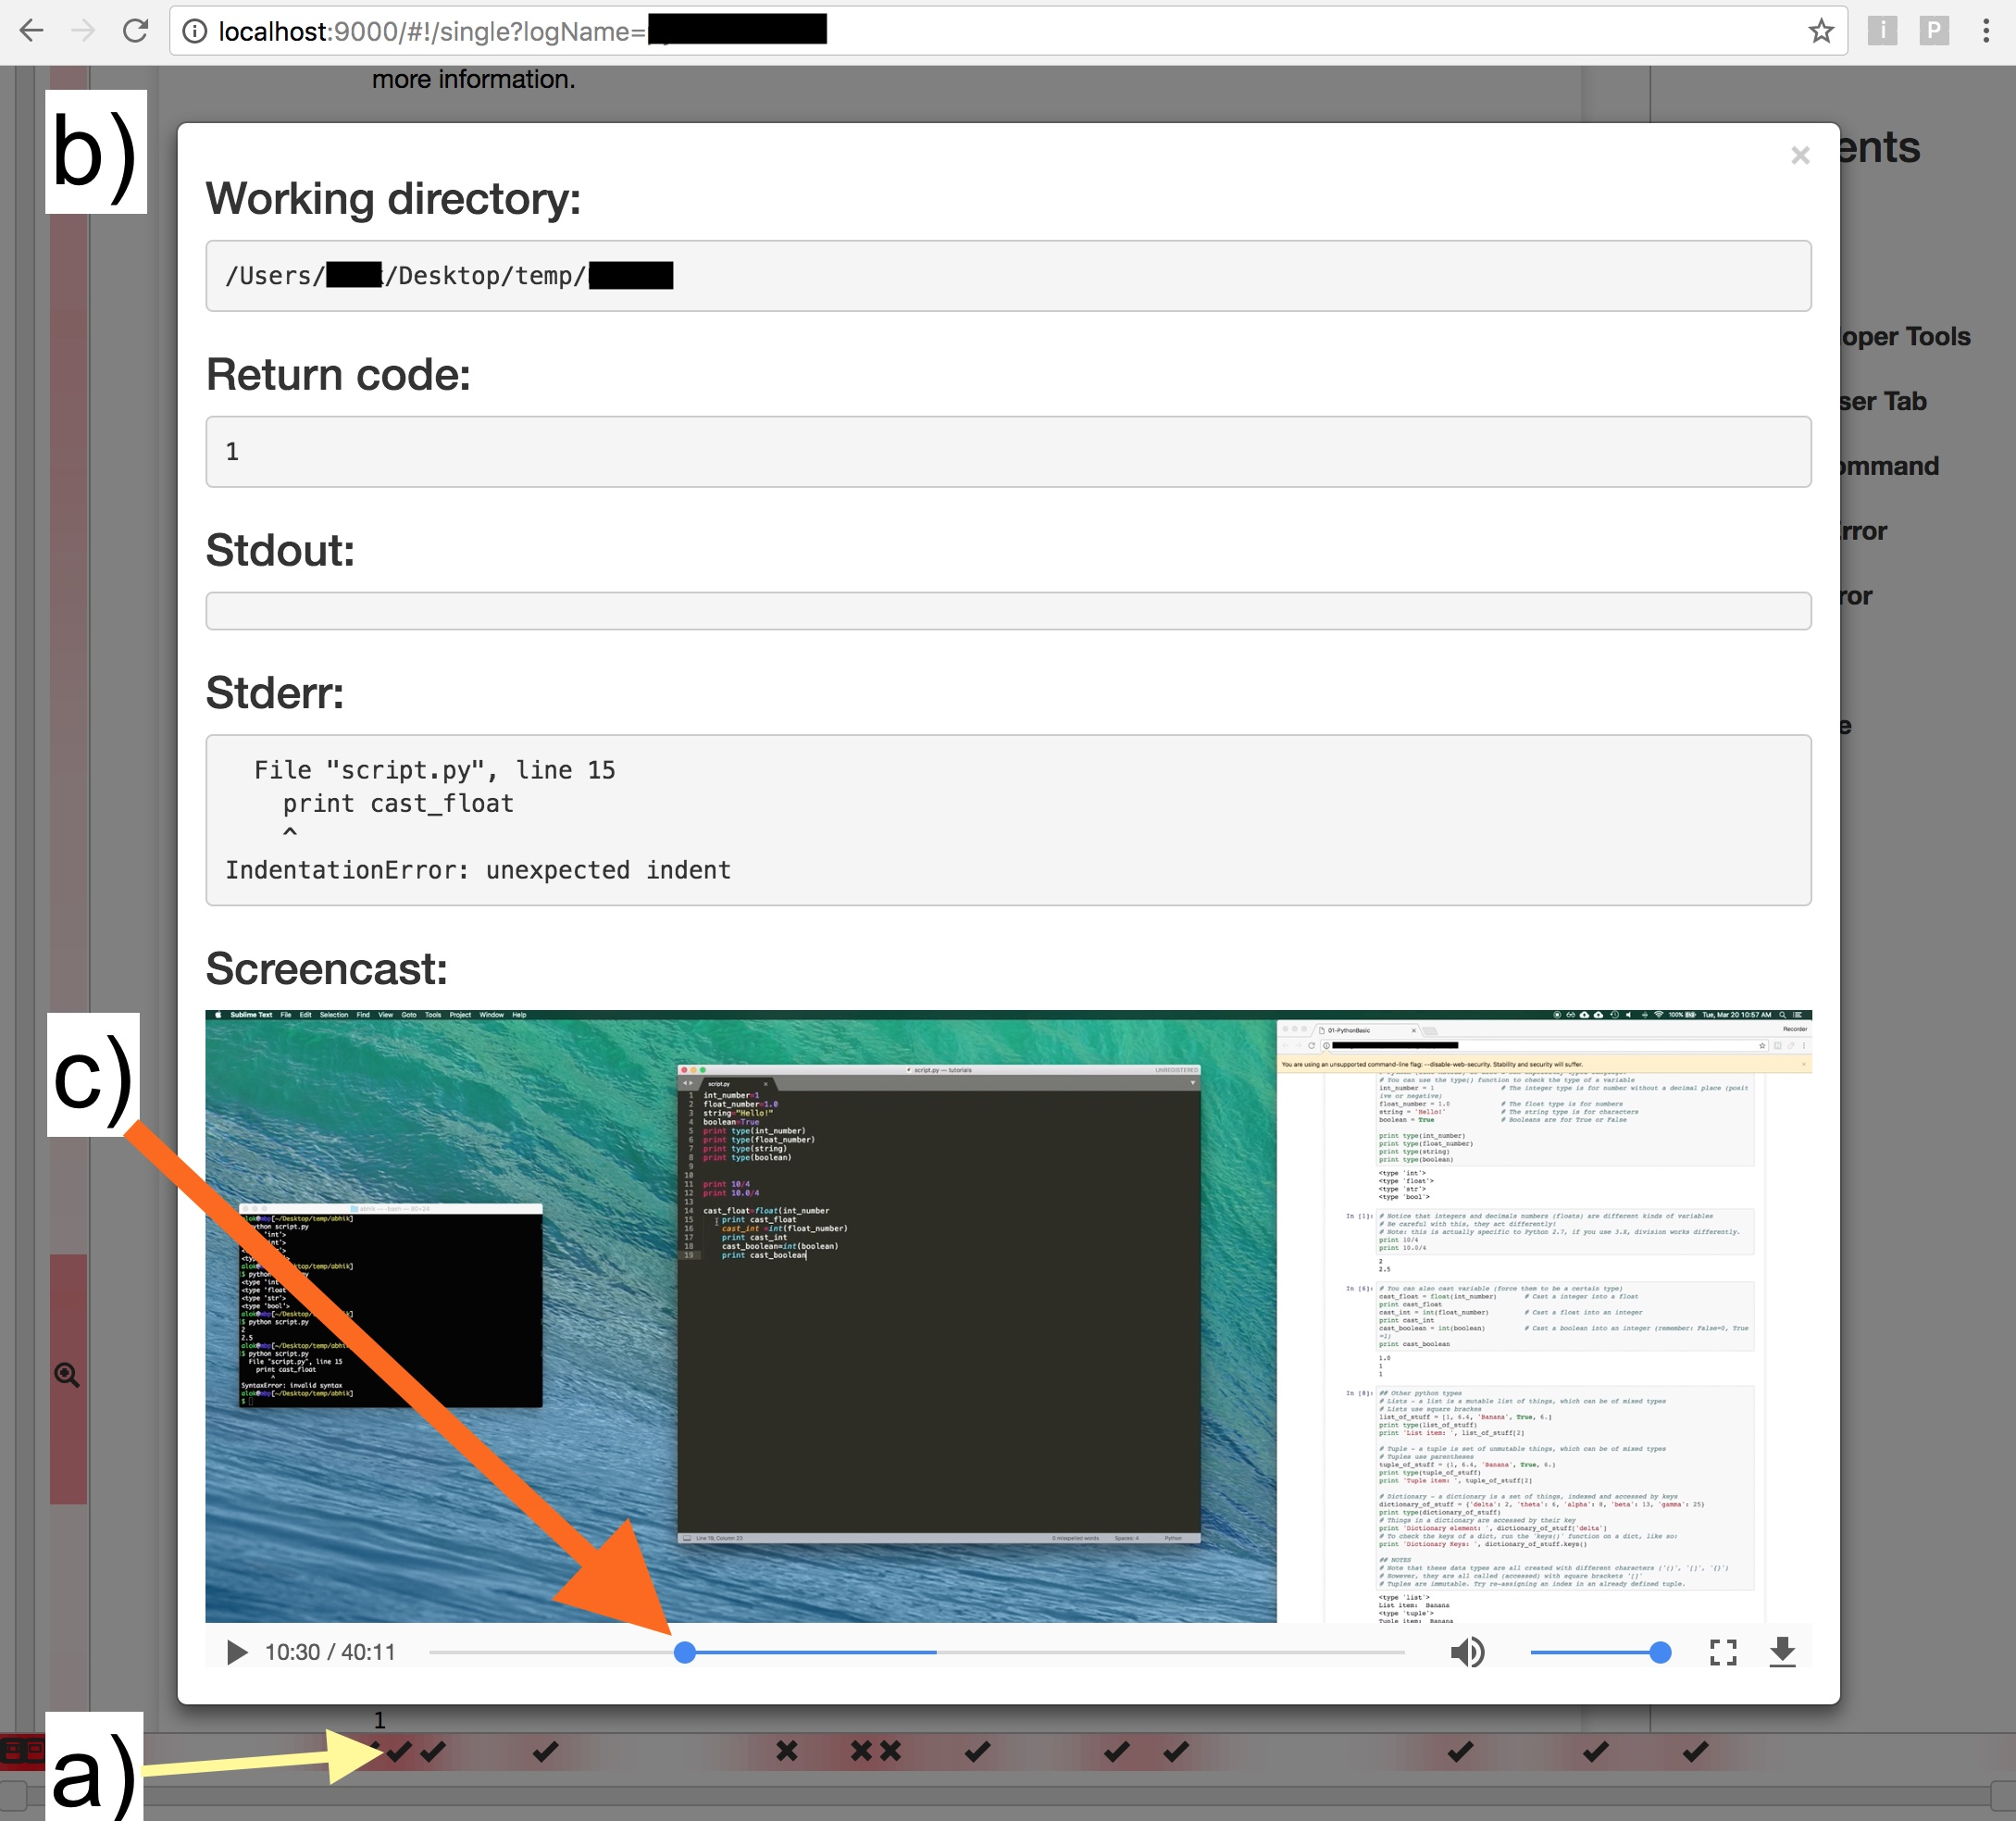
\includegraphics[width=0.95\columnwidth]{figures/porta/popup.jpg}
  %\vspace{-0.25em} % stent

  \caption{Event markers and pop-ups: a) When the user clicks on an
  event marker on a heatmap, Porta will b)~pop up a dialog showing
  details about that event. c)~This dialog also includes a fullscreen video
  of the test session that starts playing 20 seconds before that event
  occurred.}

  \label{fig:popup}
  \vspace{-0.5em} % stent
\end{figure}


Similarly, a \emph{temporal heatmap} along the bottom of the
tutorial webpage shows the density of events
logged from \tab{tbl:tracers} throughout the time duration of the
testing session. This lets viewers get a sense for the temporal ordering
of events in the testing session and filter by time ranges (described later).

\textbf{Event markers and pop-ups}: Heatmaps show an overview of the
session's activity, but it is also important to see exactly which
actions the participant performed while they were focusing on each part
of the tutorial. To surface this data, Porta displays an \emph{event
marker} for each type of event in \tab{tbl:tracers} at the approximate
webpage location where the user was looking when they performed that
action. When mouse hover data is available, this marker is placed at the
center of the focused DOM element; when it is not available, the marker
is placed at the center of the viewport's vertical position. An
identical copy of that marker appears on the temporal heatmap as well.

When the user clicks on an event marker on either the positional or
temporal heatmap (\fig{fig:popup}a), a pop-up dialog appears to show the
details of that event (\fig{fig:popup}b). This dialog contains an
embedded screencast video recording of the entire session with its seek
position set to 20 seconds prior to that event's occurrence
(\fig{fig:popup}c). This way, viewers can see the context leading up to
the selected event.

It also displays more detailed contextual data depending on
event type (\fig{fig:popup}b): Clipboard events show the textual contents that were copied
at the time of occurrence. Shell commands, toolchain invocations, and
remote ssh invocations show all of the logged data, including
command-line arguments, textual outputs, error messages, return codes,
and the contents of the affected files at the time
that command was run. Likewise for browser actions: If a new webpage tab
or window was opened, it shows that page's URL; if any JavaScript errors
arose, those are also shown.

If an event occurred when an embedded video on the tutorial
webpage was playing (or was paused at a non-starting position), then its
pop-up dialog also displays a video player that loads that video at the same position.
This level of detail is important for
video-centric tutorials: Without it, viewers can see only that the event
occurred when the mouse was hovering over an embedded video element on
the tutorial webpage, but not where the participant was watching \emph{within
the video} when they performed an action that logged that event.


\textbf{Filtering to reduce visual overload}:
%
By default all events are shown on both the positional and temporal
heatmaps. Although their positions are slightly jittered to prevent
direct overlap, if there are too many events, it may still be hard to
select individual markers. To mitigate this problem, Porta allows
viewers to filter by event type using facets (checkboxes), which will
show only selected kinds of events on heatmaps.

Viewers can also filter by time. By dragging a double-ended range
slider on the temporal heatmap, they can hone in on a time range. This
will show markers for only events that occurred within that range in
\emph{both} the temporal and positional heatmaps. It will also re-render the
positional heatmap to show the relative amounts of time that the
participant viewed portions of the webpage during that selected time
range.

Viewers can also filter by position using a similar double-ended range
slider on the positional heatmap. This will again filter events on
both heatmaps to show only those within the selected range.
%
Another benefit of positional filtering is being able to zoom in on a
detailed heatmap about a specific portion of the webpage.
%
One limitation of showing a single global heatmap that spans the entire
webpage is that certain regions may be too close in value and thus
appear almost as the same color. When the user selects a positional
range, the heatmap will be computed only for vertical positions within
that range, which will amplify those subtle value differences.


\textbf{Aggregating multiple sessions}: Porta can aggregate the data
collected from multiple test sessions in a simple way. It overlays all
of the trace data on the positional heatmap so that it visualizes the
relative amounts of time spent by all participants on each portion of
the tutorial webpage. This is akin to a source code profiler showing
aggregated results from multiple independent executions. Likewise, event
markers from all participants are shown on the heatmap. To avoid further
visual overload, Porta adds an additional facet so that the viewer can
filter by participant ID as well as by event type.
%\todo{add participant and event type facets to a screenshot to clarify}

We chose not to display a temporal heatmap when aggregating multiple
sessions since each participant likely takes differing amounts of time to
work through the tutorial and perform their actions in different
orders.
%
An alternative design is to display separate temporal heatmaps for each
participant, but that may lead to even more visual overload.
%
If a viewer wants to inspect an individual participant's session in
detail, they can view it in isolation in its own browser window.
